\subsection{Side muon range detector}
Two Side-MRD modules will be constructed by the end of January 2018. 
Each Side-MRD module is composed of iron plates and scintillator bars for tracking secondary particles from neutrino interactions. 
Support structure of the Side-MRD module mainly consists of 11 steel plates of which dimensions are $1800\times1610\times30$ mm$^{3}$, is sized as $2236\times1630\times975$ mm$^{3}$ as shown in Figure \ref{fig:side_mrd_support_structure}, and weights $\sim$8.5 ton. 
80 scintillator bars are installed in one Side-MRD module, and each scintillator bar is sized as $1800\times200\times7$ mm$^{3}$ including reflector part. 
Scintillation light is collected by wave length shifting fibers, Y-11 (S type) with a diameter of 1.0 mm produced by Kuraray. 
The fiber is glued by optical cement in a S-shape groove on the surface of the scintillator bar as shown in Figure \ref{fig:side_mrd_scintillator}. 
Two optical connectors are attached to either end of the fiber, and scintillation light is lead to two MPPCs, S13081-050CS(X1), produced at Hamamatsu Photonics. 
For each MPPC, 667 pixels of APD are aligned in a shape of square 1.3 mm on a side. 

\begin{figure}[tbh]
\begin{center}
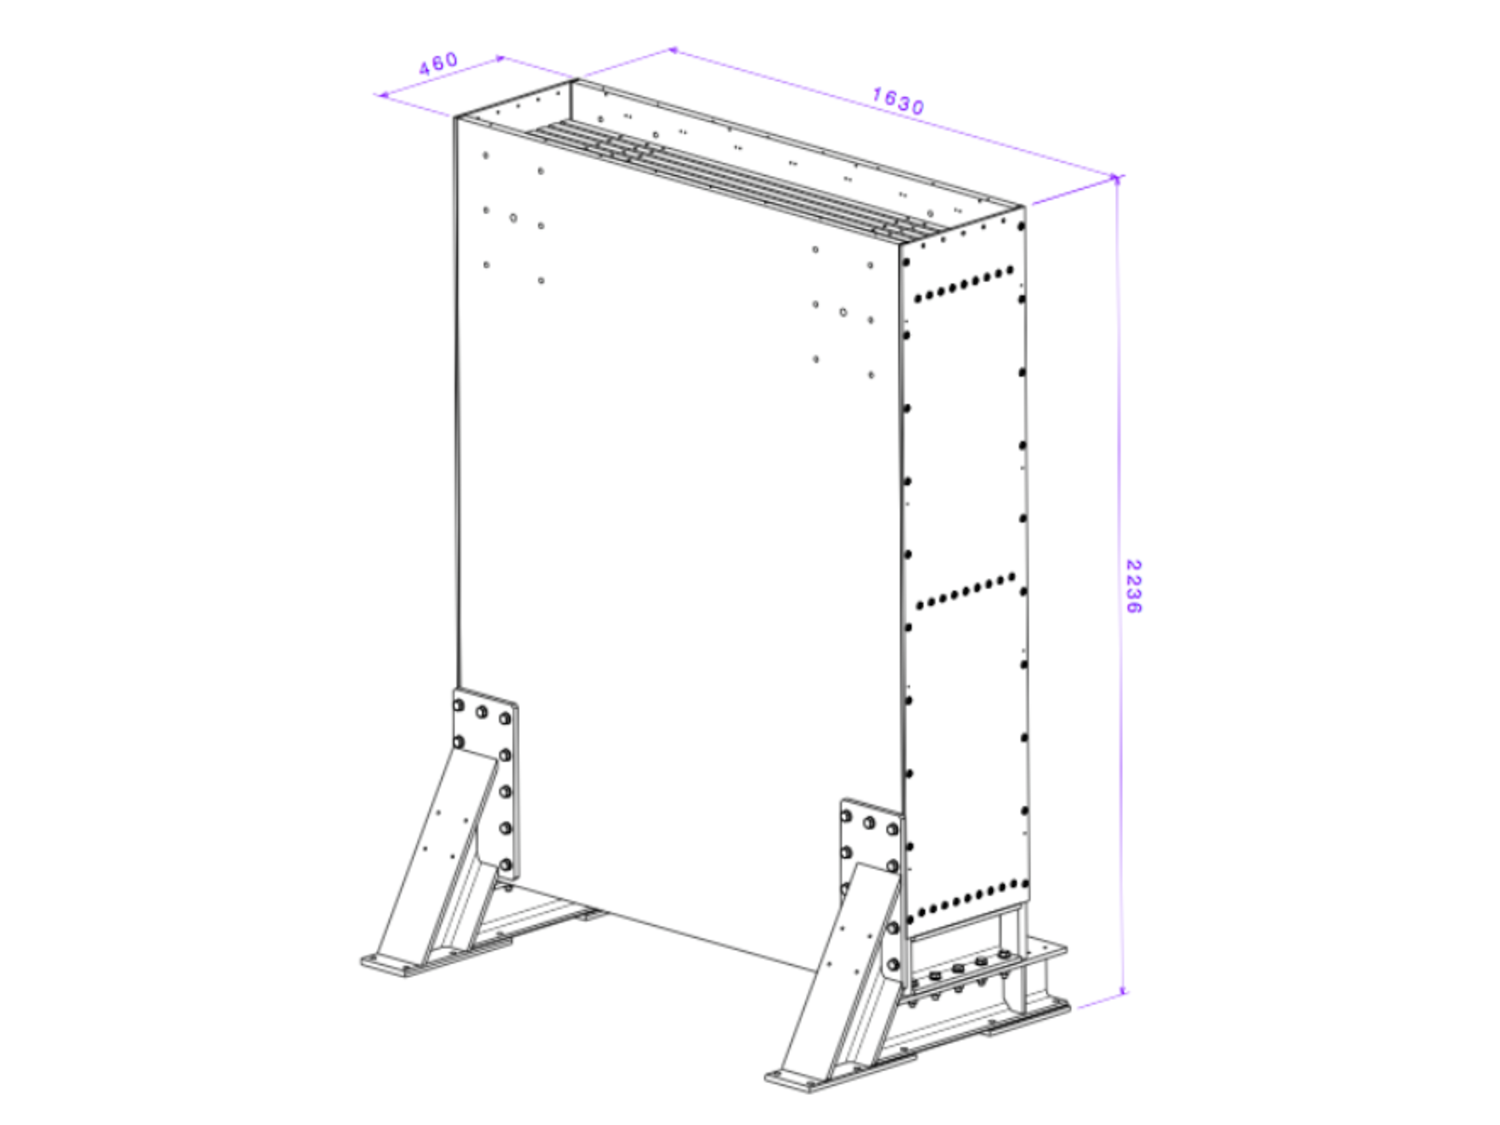
\includegraphics[width=0.8\linewidth]{fig/side_mrd_structure.pdf}
\end{center}
\caption{
Support structure of the Side-MRD module.
}
\label{fig:side_mrd_support_structure}
\end{figure}

\begin{figure}[tbh]
\begin{center}
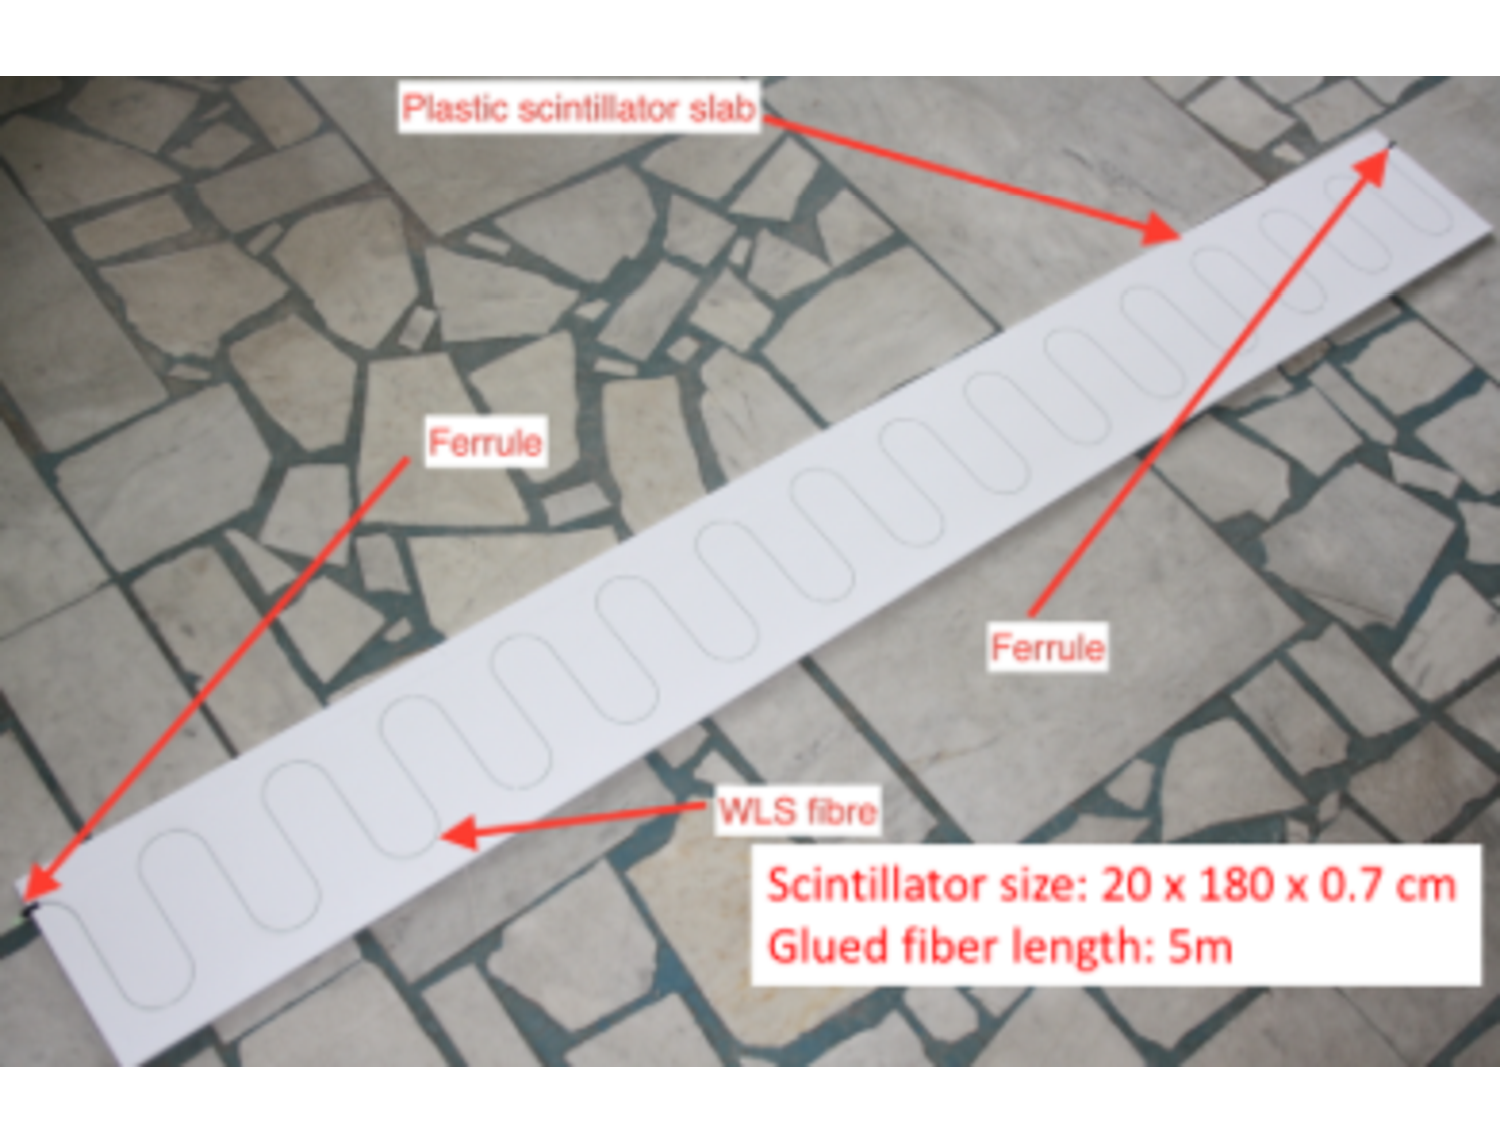
\includegraphics[width=0.8\linewidth]{fig/side_mrd_scintillator.pdf}
\end{center}
\caption{
Scintillator bar of the Side-MRD modules.
}
\label{fig:side_mrd_scintillator}
\end{figure}


Construction of scintillator bars of the Side-MRD modules had been completed in Russia, and they were transported to Japan in July 2017. 
Construction of Side-MRD modules will be done from November 2017 to January 2018 at Yokohama National University, then they will be transported to J-PARC and will be installed to the B2 floor of the T2K near detector hall before staring the T2K beam in March 2018.
